% ---
\chapter{Conceitos, definições e resultados fundamentais em compressão de dados}
% ---
Este capítulo apresenta algumas definições, conceitos e resultados fundamentais para o entendimento das técnicas de compressão que serão discutidas em capítulos posteriores.

% -- Definições básicas de código
\section{Código}

Dado um conjunto $A$, usaremos a notação $A^+$ para definir o conjunto
que contém todas as cadeias não-vazias formadas pelas possíveis
combinações de $A$. Ou seja,
\begin{equation*}
  \emph{A}^+ = \Big\{
  (a_1,a_2,\dotsc, a_n) \colon n\in\mathbb{N}, \ n>0,
  \ a_i \in A \ \forall i \in \{1,\dotsc,n\} 
  \Big\}
\end{equation*}
Por simplicidade de notação, utilizaremos $a_1a_2\dotsm a_n$ para
denotar a sequência $(a_1,a_2,\dotsc, a_n)$ quando não houver
ambiguidade.

Um \textbf{alfabeto} $A$ é um conjunto finito. Chamaremos os elementos
de $A$ de \textbf{símbolos} ou \textbf{letras} e os elementos de $A^+$
de \textbf{cadeias} ou \textbf{palavras}.

Um \textbf{código} $C$ mapeia cada símbolo $m \in M$ para uma cadeia
em $W^+$. Mais precisamente, um código é uma função injetora de um
conjunto $M$ para $W^+$. O conjunto $M$ é chamado de \textbf{alfabeto
  de origem} e $W$ é chamado de \textbf{alfabeto código}. Chamaremos
cada cadeia na imagem de $C$ de \textbf{palavra-código}.

Dentro deste contexto, definimos o \textbf{comprimento} de uma palavra
$w\in W^+$, denotado por $l(w)$, como o inteiro positivo que
representa o tamanho da sequência $w$.

Tome como exemplo o alfabeto de origem $M = \{a, b, c\}$ e o alfabeto
código $W = \{0, 1\}$ composto somente por valores binários,
poderíamos definir um código $C$ da seguinte forma:

\begin{table}[!h]
   \centering
   \caption{Tabela do código C} \label{tab:vcode}
   \begin{tabular}{|l|c|c|c|c|c|c|r|}
        \hline
        \small{alfabeto de origem} & \small{palavra-código} \\ \hline
              a &   1   \\ \hline
              b &   01  \\ \hline
              c &   00  \\ \hline
  \end{tabular}
\end{table}
Neste exemplo, o \textbf{comprimento} da palavra-código associado à
letra ``b''~é dado por $l(C(b)) = l(01) = 2$.

As palavras-código associadas a cada símbolo podem ter um tamanho \emph{fixo} ou \emph{variável}.
Códigos nos quais palavras-código possuem um comprimento fixo são chamados de \textbf{códigos de comprimento fixo}, enquanto os que possuem alfabetos de comprimento variáveis são chamados \textbf{códigos de comprimento variável}. Note que o exemplo anterior é um código de comprimento variável. 
Provavelmente o exemplo mais conhecido de código de \textbf{comprimento fixo} seja código ASCII, que mapeia 64 símbolos alfa-numéricos (ou 256 em sua versão estendida) para palavras-código de 8 bits. 
Todavia, no contexto de compressão de dados procuramos construir códigos que podem variar em seu comprimento baseados na sua probabilidade associada, a fim de reduzir o tamanho médio da \emph{string} original ao codificá-la.

\subsection{Códigos unicamente decodificáveis e livres de prefixo}

%Um código é \textbf{distinto} se pode ser representado como uma função \textbf{bijetora}, i.e, $\forall$ $m_1$, $m_2$ $\in$ M, \emph{C($m_1$)} $\neq$ \emph{C($m_2$)}.
Dado um alfabeto de origem $M$, chamamos as palavras em $M^+$ de
\textbf{mensagens}. De fato, queremos codificar e decodificar
mensanges utilizando códigos e não somente símbolos isolados. Podemos
estender código para mensagens naturalmente da forma a seguir. Dado um
código $C\colon M\to W^+$, defina \textbf{código estendido} $C^+: M^+\to W^+$ por
\begin{equation*}
  C^+(m_1m_2\dotsc m_k) =
  \textrm{concat}(C(m1),C(m_2),\dotsc,C(m_k)), \text{ para todo }m_1m_2\dotsc m_k\in M^+,
\end{equation*}
onde $\textrm{concat}(\cdot)$ é a função de concatenação de sequências.


Um código $C\colon M\to W^+$ é dito \textbf{unicamente decodificável}
se $C^+$ é uma função injetora. Ou seja, toda mensagem é mapeada para
uma palavra única.

Um \textbf{código livre de prefixo} é um código em que nenhuma
palavra-código é prefixo de outra. Uma palavra $w_1\dotsm w_k$ é
\textbf{prefixo} de uma palavra $v_1\dotsm v_\ell$ se $k\leq \ell$ e
$w_1\dotsm w_k = v_1\dotsm v_k$. Ou seja, um código $C\colon M\to W^+$
é livre de prefixo se vale que, para quaisquer $m,m' \in M$ distintos,
$C(m)$ não é prefixo de $C(m')$.

Por exemplo, o código que possui sua imagem no conjunto de
palavras-código \emph{$W^+$} := $\{1, 01, 000, 001\}$ não possui
nenhuma cadeia que é prefixo de outra, portanto é considerado um
\textbf{código livre de prefixo}.  Códigos livres de prefixo não
apenas são unicamente decodificáveis como podem ser
\emph{decodificados instantaneamente}, pois, ao processar uma cadeia
de sequência de palavras-código podemos decodificar cada uma delas sem
precisar verificar o início da seguinte.

Todo código $C\colon M\to W^+$ pode ser representado por uma árvore
$T(C)$ onde
\begin{itemize}
\item as arestas são rotuladas por símbolos de $W$ e,
\item cada símbolo $m \in M$ é associado a um nó $v(m)$ da árvore,
\item para cada símbolo $m\in M$, a palavra-código $C(m)$ é obtida
  pelo caminho da raiz até $v(m)$ através da concatenação dos rótulos
  das arestas do caminho
\item cada folha da árvore é $v(m)$ para algum $m\in M$.
\end{itemize}
Note que, se $C$ é um código livre de prefixo, todos os símbolos em
$M$ são mapeados para folhas, pois se $v(m)$ está no caminho da folha
até $v(m')$ ($v(m)$ é ancestral de $m'$), então $C(m)$ é prefixo de
$C(m')$. A árvore a seguir representa o código da
Tabela~\ref{tab:vcode} (claramente um código livre de prefixo).

\begin{figure}[h]
   \centering
   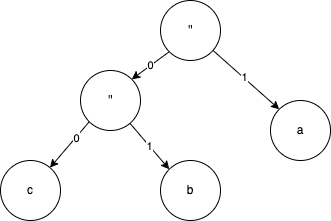
\includegraphics[scale=0.75]{figs/prefixtree.png}
    \caption{Árvore de um código livre de prefixo}
    \label{fig:prefixt}
 \end{figure}
% ----------------------------------------------------------------------------
% Probabilidade -------------------------
\section{Relações fundamentais com a Teoria da Informação}
A codificação é comumente divida em duas componentes diferentes: \emph{modelo} e \emph{codificador}. 
O \emph{modelo} identifica a distribuição de probabilidade das mensagens baseado em sua semântica e estrutura. 
O \emph{codificador} toma vantagem de um possível \emph{enviesamento (bias)} apontado pela modelagem, e utiliza as probabilidades associadas para reduzir a quantidade de dados necessária para representar a mesma informação (substituindo os símbolos que ocorrem com maior frequência por palavras-código menores).
Isso significa que, a codificação está diretamente ligada às probabilidades associadas a cada símbolo do alfabeto de origem.

Nesta seção, vamos construir o embasamento teórico necessário para entender a relação entre as probabilidades associadas e o comprimento das mensagens, e consequentemente criar uma noção dos parâmetros que devem ser maximizados ou minimizados para alcançar uma codificação eficiente.

\subsection{Conceitos básicos em Probabilidade}
Neste texto, iremos trabalhar com espaços de probabilidade finitos,
pois lidamos com alfabetos de origem finitos. Um \textbf{espaço de
  probabilidade finito} é um par $(\Omega, P)$, onde $\Omega$ é um
conjunto finito e $P\colon \Omega \to \mathbb{R}_{\geq 0}$ tal que
$\sum_{\omega \in \Omega} P(\omega) = 1$.

O conjunto $\Omega$ é chamado de \textbf{espaço amostral} e $P$ é
chamada de \textbf{função de probabilidade}. Um \textbf{evento} $E$ é
um sunconjunto de $\Omega$ e sua probabilidade é definida como $P(E)
:= \sum_{\omega \in E} P(\omega)$.

Uma \textbf{variável aleatória} $X$ associa um número real a cada
um dos elementos de $\Omega$. Em outras palavras, $X$ é uma
função que mapeia os elementos do espaço amostral para números
reais. Uma variável aleatória é chamada \textbf{discreta} quando os
valores dos experimentos associados a ela são números finitos ou ao
menos infinitos que podem ser contados.

Podemos descrever melhor uma variável aleatória $X$, atribuindo
probabilidades sobre os valores que esta pode assumir. Esses valores
são atribuídos pela \textbf{distribuição de probabilidade}, denotada
por $p_X$, definida para cada $x\in\mathbb{R}$ como
\begin{equation} \label{eq:dist_prob_def}
p_X(x) = P(\{\omega\in \Omega: X(\omega) = x\}).
\end{equation}
Por simplicidade, de notação utilizamos $P(X=x)$ para denotar
$P(\{\omega\in \Omega: X(\omega) = x\})$. Note que a pré-imagem de $X$
é o espaço amostral e, portanto,
\begin{equation} \label{eq:dist_prob_sum}
\sum_{x ~\in ~im_X}^{}p_X(x) = 1,
\end{equation}
onde $im_X$ denota a imagem de $X$.

O \textbf{valor esperado} (ou \textbf{esperança}) da variável aleatória $X$ é definido como
\begin{equation} \label{eq:exp_val}
\textbf{E}[X] = \sum_{x ~\in ~im_X}^{} xp_X(x).
\end{equation}
%--------------------------------------
% ------------------------------ Entropia
\subsection{Comprimento médio do código}
Seja $p$ a distribuição de probabilidade associada ao alfabeto de
origem $M$. Seja $C: M \to W^+$ um código. Definimos o
\textbf{comprimento/tamanho médio} de $C$ como:
\begin{equation} \label{eq:code_len}
l_a (C) = \sum_{m \in M}^{} p(m) l(C(m)) = \mathbf{E}[l\circ C].
\end{equation}

Estamos interessados em códigos unicamente decodificáveis com o menor
comprimento médio possível. Dada um espaço de probabilidade $(M, P)$ e
um alfabeto código $W$, Um código $C: M \to W^+$ unicamente
decodificável é \textbf{ótimo} se $l_a(C)$ é mínimo, isto é, para
qualquer código unicamente decodificável \emph{C'} temos que
\begin{equation} \label{eq:code_len_optimal}
l_a(C) \leq l_a(C').
\end{equation}
Assim, temos o seguinte problema de otimização
\begin{equation} \label{eq:prog_code_len}
  \begin{array}{rl}
    \min & l_a(C)\\
    \text{sujeito a} &C: M \to W^+ \text{ é um código unicamente decodificável}
  \end{array}
\end{equation}


\subsection{Entropia}
A \textbf{entropia de Shannon} aplica as noções de entropia física
(que representa a aleatoriedade de um sistema) à Teoria da
Informação. Dada uma variável aleatória $X$ com distribuição de
probabilidade $p$, definimos \textbf{entropia} de $X$ como
\begin{equation} \label{eq:entropy}
H(X, p, b) = \sum_{x \in im_X}^{} p(x) \log_b \frac{1}{p(x)},
\end{equation}
onde $b$ é comumente tomado como $2$, mas pode assumir valores inteiros maiores do que~$2$.

Por esta definição temos que quanto menor o enviesamento da função de distribuição de probabilidade relacionada ao sistema, maior a sua entropia. Em outras palavras, a entropia de um sistema esta intimamente ligada a sua ``desordem''.

Shannon~\ref{} aplica o mesmo conceito de entropia no contexto da Teoria da Informação, ``substituindo'' o conjunto de estados pelo conjunto de símbolos $M$, isto é, $M$ é interpretado como um conjunto de possíveis símbolos, tendo como $p(m)$ a probabilidade de cada $m \in M$.
Baseado na mesma premissa, Shannon mede a informação de cada símbolo da seguinte forma
\begin{equation} \label{label:info_quantity}
\emph{i(m,b)} = \log_b \frac{1}{p(m)}.
\end{equation}

\subsection{Comprimento de Código e Entropia}
Nas seções anteriores, o comprimento médio de um código  foi definido em função da distribuição de probabilidade associada ao seu alfabeto de origem.
Da mesma forma, as noções de \textbf{entropia} relacionada a um conjunto de mensagens, têm ligação direta com as probabilidades associadas a estas. 
A seguir, será mostrado como podemos relacionar o comprimento médio de um código a sua entropia através da \textbf{Desigualdade de Kraft-McMillan} , e por consequência estabelecer uma relação direta entre \textbf{a entropia de um conjunto de mensagens e a otimalidade do código associada a estas mensagens}.

\begin{theorem}[Desigualdade de Kraft-McMillan]
  \label{thm:kraftmc}
  Sejam $M$ e $W$ conjuntos finitos tais que $|W|\leq 2$. Seja $b :=
  |W|$. Para todo código unicamente decodificável $C: M \to W^+$, vale
  que
  \begin{equation}
    \label{eq:cond_kraft_nec}
    \sum_{m\in M} b^{-l(C(m))} \leq 1.
  \end{equation}
  Além disso, para toda função $f: M\to\mathbb{N}$ tal que
  que satisfaça
  \begin{equation}
    \label{eq:cond_kraft_suf}
    \sum_{m \in M} b^{-f(m)} \leq 1,
  \end{equation}
  existe um código livre de prefixo (e, portanto, unicamente
  decodificável) tal que $l(C(m)) = f(m)$ para todo $m\in M$.
\end{theorem}

Antes de apresentar a demonstração do teorema~\ref{thm:kraftmc}, vamos
explorar as suas consequências para comprimentos de códigos
ótimos. Uma de suas consequências principais é que o valor da solução
ótima para o problema de otimização~\ref{eq:prog_code_len}
\begin{equation*} 
  \begin{array}{rl}
    \min & l_a(C) = \sum_{m\in M} p(m) l(C(m))\\
    \text{sujeito a} &C: M \to W^+ \text{ é um código unicamente decodificável}
  \end{array}
\end{equation*}
é igual ao valor ótimo do seguinte problema de otimização
\begin{equation*} 
  \begin{array}{rl}
    \min & \sum_{m\in M} p(m) f(m)\\
    \text{sujeito a} &\sum_{m \in M} b^{-f(m)} \leq 1\\
    & f:M\to\mathbb{N}
  \end{array}
\end{equation*}
Além disso, se $f^*$ é uma solução ótima para o problema acima, então
existe um código $C^*: M \to W^+$ livre de prefixo para o qual $f^*$
determina os comprimentos de suas palavras-código. Portanto, podemos
concluir que dentro os códigos unicamente decodificáveis de
comprimento médio ótimo sempre existe um que é livre de prefixo.
 
Vamos ver, em capítulos posteriores, que o algoritmo de Huffman produz
um código livre de prefixo que é ótimo dentre os códigos livres de
prefixo. A discussão acima mostra que tal código também é ótimo dentre
todos os códigos unicamente decodificáveis.

A seguir apresentamos a demonstração da Desigualdade de
Kraft-McMillan.

\begin{proof}[Prova do Teorema~\ref{thm:kraftmc}]
    Primeiramente, mostraremos a equação~\eqref{eq:cond_kraft_nec}.
    
    Seja $C:M\to W^+$ um código unicamente decodificável. Seja $b :=
    |M|$. Seja $l_{\max} = \max_{m\in M} l(C(m))$. Seja $k$ um inteiro
    positivo. Seja
    \begin{equation*}
      W_k := \left\{ C^+(m_1\dotsm m_k):
      m_1,..., m_k \in M\right\}
    \end{equation*}
    e seja
    \begin{equation*}
      W_{k,j} := \left\{
      w \in W_k: l(w) = j
      \right\},
    \end{equation*}
    para $j\in \mathbb{N}$. Temos que
    \begin{align*}
      \left(\sum_{m\in M} b^{-l(C(m))}\right)^k
      &= \prod_{i=1}^k \sum_{m_i \in M} b^{-l(C(m_i))} \\
      &= \sum_{m_1,..., m_k \in M} b^{-\sum_{i=1}^{k} l(C(m_i))} \\
      &= \sum_{w\in W_k} b^{-l(w)}\\
      &= \sum_{j=1}^{k \cdot l_{\max}} |W_{k,j}| \cdot b^{-j}\\
      &\leq \sum_{j=1}^{k \cdot l_{\max}} b^j \cdot b^{-j},
      \quad\text{ pois }|W_{k,j}|\leq b^j\\
      & = k \cdot l_{\max}
    \end{align*}
Logo,
\begin{equation*}
\sum_{m\in M} b^{-l(C(m))} \leq (k \cdot l_{max})^ \frac{1}{k},
\end{equation*}
para todo $k$ inteiro positivo. Como $\lim_{k\to\infty} (k \cdot l_{max})^ \frac{1}{k} = 1$, temos que
\begin{equation*}
\sum_{m\in M} b^{-l(C(m))} \leq 1.
\end{equation*}

\textbf{Desigualdade de Kraft}
Sem perda de generalidade, suponha que os elementos de \emph{L} estão ordenados de maneira em que:
\begin{align*}
l_1 \leq l_2 \leq ... \leq l_n
\end{align*}
Agora vamos construir um código livre de prefixo em uma ordem crescente de tamanho, de maneira em que $l(w_i) = l_i$. Sabemos que um código é livre de prefixo se e somente se ,existe uma palavra-código $w_j$  tal que nenhuma das palavras-código anteriores $(w_1, w_2, w_{j-1})$ são prefixo de $w_j$.

Sem as restrições de prefixo, uma palavra-código de tamanho $l_j$ poderia ser construída de $2^{l_j}$ maneiras diferentes. Com a restrição apresentada anteriormente, considerando uma palavra $w_k$ anterior a $w_j$ (i.e, $k < j$), existem $2^{l_j - l_k}$ possíveis palavras-código em que $w_k$ seria um prefixo, e que portanto não podem pertencer ao código. Chamaremos tal conjunto de "palavras-código proibidas". Vale notar que os elementos do conjunto de palavras-código proibidas são excludentes entre si, pois se duas palavras-código menores que \emph{j} fossem prefixo da mesma palavra-código, elas seriam prefixos entre si. 

Dito isto, podemos definir o tamanho do conjunto de palavras-código proibida para $w_j$.
\begin{equation*}
\sum_{i=1}^{j-1} 2^{l_j - l_i}
\end{equation*}

A construção do código livre de prefixo é possível se e somente se, existir ao menos uma palavra-código de tamanho $j > 1$ que não está contida no conjunto das palavras-código proibidas.
\begin{equation*}
2^{l_j} > \sum_{i=1}^{j-1} 2^{l_j - l_i}
\end{equation*}

Como o domínio do problema apresentado está restrito aos inteiros não negativos, podemos afirmar que:
\begin{align*}
2^{l_j} > \sum_{i=1}^{j-1} 2^{l_j - l_i} &= 2^{l_j} \geq \sum_{i=1}^{j-1} 2^{l_j - l_i} + 1 \\
&= 2^{l_j} \geq \sum_{i=1}^{j} 2^{l_j - l_i} \\
&= 1 \geq \sum_{i=1}^{j} 2^{-l_i} \\
&=  \sum_{i=1}^{j} 2^{-l_i} \leq 1
\end{align*}

Substituindo \emph{n} em \emph{j}, chegamos a desigualdade de Kraft.
\begin{equation*}
\sum_{l \in L}^{} 2^{-l} \leq 1.
\end{equation*}

Note que os argumentos utilizados para a construção da prova possuem dupla-equivalência, portando concluem a prova nos dois sentidos.

\end{proof}

A seguir vamos ver a relação de entropia com comprimento médio
ótimo. Primeiramente, veremos que a entropia é um limitante inferior
para o comprimento médio de códigos unicamente decodificáveis.

\begin{lemma}[Entropia como limite inferior]
  \label{lem:entropia_inf}
  Dados um conjunto finito $M$ e uma função de probabilidade $p$ para
  $M$, vale que
\begin{equation*}
  H(M, p, b) \leq l_a(C),
\end{equation*}
para todo código unicamente decodificável $C:M\to W^+$ tal que $|W| =
b$.
\end{lemma}

Po outro lado, veremos também que um código de comprimento médio ótimo
tem valor no máximo a entropia somada com $1$.

\begin{lemma}[Entropia como limite superior]
  \label{lem:entropia_sup}
  Dados um conjunto finito $M$ e uma função de probabilidade $p$ para
  $M$, existe um código $C:M\to W^+$ livre de prefixo tal que
  \begin{equation*}
    l_a(C) \leq H(M, p, b) + 1
  \end{equation*}
  onde $b = |W|$.
\end{lemma}

  A seguir apresentamos as demonstrações dos lemas acima.
  
  \begin{proof}[Prova do Lema~\ref{lem:entropia_inf}]
    Seja $C:M\to W^+$ um código unicamente decodificável e seja $b :=
    |W|$. Seja $p$ uma função de probabilidade para $M$. Queremos
    provar que $H(M, p,b) - l_a(C) \leq 0$.

    Substituindo $H(M,p, b)$ e $l_a(C)$ por suas definições
    (equação~\eqref{eq:entropy} e equação~\eqref{eq:code_len}, resp),
    temos
    \begin{align*}
      H(M, p, b) - l_a(C)
      &=
      \sum_{m \in M} p(m) \log_b \frac{1}{p(m)}
      - \sum_{m \in M}^{}p(m) l((C(m))) \\
      &=
      \sum_{m \in M} p(m) \left(
      \log_b \frac{1}{p(m)} - l(C(m))
      \right) \\
      &=
      \sum_{m \in M} p(m) \left(
      \log_b \frac{1}{p(m)} - \log_b b^{l((C(m)))}
      \right) \\
      &= \sum_{m \in M}^{}p(m) \log_b \left(\frac{b^{-l(C(m))}}{p(m)}\right)
    \end{align*}

    Pela desigualdade de Jensen, se uma função $f:M\to\mathbb{R}$ é
    côncava, então $\sum_{m\in M} p(m) f(x_m) \leq f(\sum_{m\in M}
    p(m)~x_m)$ para quaisquer $x_m$ positivos. Como a função $\log_b$
    é côncava, podemos aplicar a desigualdade de Jansen ao resultado
    obtido anteriormente para deduzir que
\begin{equation*}
  \sum_{m \in M}^{}p(m) \log_b  \left(\frac{b^{-l(C(m))}}{p(m)}\right)
  \leq
  \log_b\left(\sum_{m \in M} b^{-l(C(m))}\right)
\end{equation*}
Agora, aplicamos a desigualdade de Kraft-McMillan, e concluímos que
\begin{equation*}
  H(M, p, b) - l_a(C)
  \leq
  \log_b 1 = 0,
\end{equation*}
como queríamos demonstrar.
\end{proof}


  \begin{proof}[Prova do Lema~\ref{lem:entropia_sup}]
    Seja $(M,p)$ um espaço de probabilidade finit. Podemos assumir que
    $p(m)>0$ para todo $M$, pois elementos de $M$ com probabilidade
    zero podem ser ignorados.

    Seja $f:M\to\mathbb{N}$ definida como $f(m) = \left \lceil{\log_b
      \frac{1}{p(m)} }\right \rceil$ para todo $m\in M$. Temos que
\begin{align*}
  \sum_{m \in M}^{} b^{-f(m)} &=
  \sum_{m \in M}^{} b^{-\left \lceil{\log_b \frac{1}{p(m)} }\right \rceil} \\
  &\leq \sum_{m \in M}^{} b^{-{\log_b \frac{1}{p(m)} }} \\
  &= \sum_{m \in M}^{} p(m) \\
  &= 1
\end{align*}
Ou seja, $f$ satisfaz a condição~\eqref{eq:cond_kraft_suf}. De acordo
com a desigualdade de Kraft-McMillan existe um código livre de prefixo
$C$ com palavras-código de tamanho dado por $f$, portanto
\begin{align*}
  l_a(C) &=
  \sum_{m \in M} p(m) f(m) \\
  &=  \sum_{m \in M} p(m) \left \lceil{\log_2 \frac{1}{p(m)} }\right \rceil \\
&\leq \sum_{m \in M}^{}p(m) \left(1 + \log_2 \frac{1}{p(m)}\right) \\
&= 1 +  \sum_{m \in M}^{}p(m) \log_2 \frac{1}{p(m)} \\
&= 1 + H(M,p,b).
\end{align*}
\end{proof}


% ------------------- End of chapter 1 -----------------------------

% --- Guardando para exemplo
% A formatação das referências bibliográficas conforme as regras da ABNT são um
% dos principais objetivos do \abnTeX. Consulte os manuais
% \citeonline{abntex2cite} e \citeonline{abntex2cite-alf} para obter informações
% sobre como utilizar as referências bibliográficas.

% %-
% \subsection{Acentuação de referências bibliográficas}
% %-

% Normalmente não há problemas em usar caracteres acentuados em arquivos
% bibliográficos (\texttt{*.bib}). Na~\autoref{tabela-acentos} você encontra alguns exemplos das conversões mais importantes. Preste atenção especial para `ç' e `í'
% que devem estar envoltos em chaves. A regra geral é sempre usar a acentuação
% neste modo quando houver conversão para letras maiúsculas.

% \begin{table}[htbp]
% \caption{Tabela de conversão de acentuação.}
% \label{tabela-acentos}

% \begin{center}
% \begin{tabular}{ll}\hline\hline
% acento & \textsf{bibtex}\\
% à á ã & \verb+\`a+ \verb+\'a+ \verb+\~a+\\
% í & \verb+{\'\i}+\\
% ç & \verb+{\c c}+\\
% \hline\hline
% \end{tabular}
% \end{center}
% \end{table}


% ---
% \section{Deu pau em algo?}
% ---

% Consulte a FAQ com perguntas frequentes e comuns no portal do \abnTeX:
% \url{https://code.google.com/p/abntex2/wiki/FAQ}.

% Inscreva-se no grupo de usuários \LaTeX:
% \url{http://groups.google.com/group/latex-br}, tire suas dúvidas e ajude a galera se tiver tudo certo.


